\documentclass[11pt]{article}
\usepackage[utf8]{inputenc}
\usepackage[T1]{fontenc}
\usepackage[brazil]{babel}
\usepackage[margin=2.3cm]{geometry}
\usepackage{booktabs}
\usepackage{amsmath}
\usepackage{caption}
\usepackage{graphicx}

\title{\textbf{Resultados — Determinantes do peso de VALE3 nos fundos Itaú (2016--2021)}}
\author{TCC — FGV EESP \\ Orientador: Prof.\ Maurício Ferraresi Jr.}
\date{\today}

\begin{document}
\maketitle

\section{Objetivo e amostra}

Estimamos como o \textbf{peso de VALE3} (participação na carteira, em fração de
0 a 1) em cada fundo da gestora Itaú é explicado por características do fundo e da
ação. É o \emph{Passo~1} da metodologia do orientador: os coeficientes da
regressão funcionam como um \textbf{fator latente} que resume, em poucos números,
como as posições dependem das características.

\medskip
\noindent\textbf{Amostra:} painel fundo $\times$ mês, \textbf{2016--2021}
(\textbf{72 meses}), gestoras Itaú (Asset Management, DTVM, Unibanco), restrito a
observações com mais de 3 cotistas (remoção de fundos exclusivos). São
\textbf{11.532 observações} fundo-mês (das quais 11.413 com fluxo disponível) e
\textbf{623 fundos} distintos. O painel completo (sem o filtro de cotistas) tem
26.123 observações.

\section{Variáveis e tratamentos}

\begin{table}[h]
\centering\small
\begin{tabular}{@{}lll@{}}
\toprule
\textbf{Variável} & \textbf{Definição} & \textbf{Tratamento} \\
\midrule
peso\_vale3 (alvo) & participação de VALE3 na carteira (fração) & nível \\
AUM & patrimônio líquido do fundo (R\$) & $\log$ \\
nº cotistas & número de cotistas & $\log$ \\
FIC & 1 se Fundo de Inv.\ em Cotas, 0 se FI & dummy \\
Fluxo/AUM & (captação $-$ resgate) do mês / AUM & razão \\
Preço VALE3 & fechamento no último pregão do mês anterior & nível (R\$, nominal) \\
Beta VALE3 & beta móvel 252 pregões vs.\ Ibovespa & nível \\
\bottomrule
\end{tabular}
\end{table}
\noindent\footnotesize Preço e beta são constantes entre fundos dentro de um mês
(variáveis agregadas) $\Rightarrow$ entram apenas na regressão \emph{pooled}, não
na cross-section mês a mês. \normalsize

\section{Tabela 1 — Cross-section mês a mês (Fama--MacBeth, 72 meses)}

Para cada mês roda-se uma regressão separada; reporta-se a \textbf{média dos 72
coeficientes mensais}, com erro-padrão calculado pela variação entre os meses
(Fama--MacBeth). ``Meses +'' = em quantos dos 72 meses o coeficiente teve sinal
positivo (estabilidade).

\begin{table}[h]
\centering
\begin{tabular}{@{}lrrrrcc@{}}
\toprule
\textbf{Variável} & \textbf{Coef.\ médio} & \textbf{EP (FM)} & \textbf{$t$} & \textbf{$p$} & \textbf{Meses +} & \textbf{Sig.} \\
\midrule
Intercepto        & $0{,}08939$  & $0{,}00413$ & $21{,}6$  & $<0{,}001$ & 72/72 & *** \\
$\log$(AUM)       & $-0{,}00376$ & $0{,}00019$ & $-19{,}3$ & $<0{,}001$ & 0/72  & *** \\
$\log$(cotistas)  & $0{,}00387$  & $0{,}00020$ & $19{,}8$  & $<0{,}001$ & 72/72 & *** \\
FIC (dummy)       & $-0{,}01697$ & $0{,}00089$ & $-19{,}2$ & $<0{,}001$ & 0/72  & *** \\
Fluxo/AUM         & $-0{,}00044$ & $0{,}00309$ & $-0{,}14$ & $0{,}886$  & 39/72 & n.s. \\
\bottomrule
\end{tabular}
\end{table}
\noindent\footnotesize $R^2$ médio por mês $= 0{,}152$. \quad *** $p<0{,}001$;
n.s.\ = não significativo. \normalsize

\subsection*{Interpretação}
\begin{itemize}
\item \textbf{$\log$(AUM) negativo (sinal estável nos 72 meses):} fundos
\emph{maiores} carregam \emph{menor} peso em VALE3 — são mais diversificados.
\item \textbf{$\log$(cotistas) positivo (72/72):} fundos com mais cotistas têm
\emph{maior} peso em VALE3.
\item \textbf{FIC negativo (0/72):} Fundos de Investimento em Cotas têm \emph{menos}
VALE3 \emph{direto} (investem via cotas de outros fundos).
\item \textbf{Fluxo/AUM não significativo:} o fluxo \emph{não explica o nível} do
peso — provavelmente explica a \emph{variação} do peso (a investigar no Passo~2).
\item \textbf{Estabilidade:} os três fatores estruturais têm sinal idêntico nos 72
meses, o que justifica modelar o coeficiente como um fator que evolui devagar
(random walk / filtro de Kalman) no Passo~2.
\end{itemize}

\section{Tabela 2 — Regressão \emph{pooled} (72 meses empilhados)}

Aqui as 11.413 observações entram juntas, permitindo incluir preço e beta
(identificados pela variação ao longo dos 72 meses).

\begin{table}[h]
\centering
\begin{tabular}{@{}lrrrrc@{}}
\toprule
\textbf{Variável} & \textbf{Estimativa} & \textbf{EP} & \textbf{$t$} & \textbf{$p$} & \textbf{Sig.} \\
\midrule
Intercepto       & $0{,}10361$  & $0{,}00407$ & $25{,}4$   & $<0{,}001$ & *** \\
$\log$(AUM)      & $-0{,}00353$ & $0{,}00019$ & $-19{,}0$  & $<0{,}001$ & *** \\
$\log$(cotistas) & $0{,}00390$  & $0{,}00013$ & $31{,}0$   & $<0{,}001$ & *** \\
FIC (dummy)      & $-0{,}01674$ & $0{,}00079$ & $-21{,}1$  & $<0{,}001$ & *** \\
Fluxo/AUM        & $-0{,}00033$ & $0{,}00034$ & $-0{,}99$  & $0{,}324$  & n.s. \\
Preço VALE3      & $0{,}000149$ & $0{,}000016$& $9{,}2$    & $<0{,}001$ & *** \\
Beta VALE3       & $-0{,}02368$ & $0{,}00142$ & $-16{,}7$  & $<0{,}001$ & *** \\
\bottomrule
\end{tabular}
\end{table}
\noindent\footnotesize $R^2 = 0{,}164$; $n = 11.413$. \quad *** $p<0{,}001$;
n.s.\ = não significativo. \normalsize

\subsection*{Interpretação}
\begin{itemize}
\item Características de \textbf{fundo} (AUM, cotistas, FIC) repetem os sinais da
cross-section e são \textbf{altamente significativas}.
\item \textbf{Preço (+, $p<0{,}001$):} meses com VALE3 mais cara $\to$ peso médio
maior. \textbf{Beta ($-$, $p<0{,}001$):} meses com VALE3 mais arriscada (beta
alto) $\to$ peso médio menor (aversão a risco).
\item Com \textbf{72 meses}, preço e beta ficam bem identificados. (No piloto de só
2016, com 12 valores, o beta saía positivo e fraco; com 72 meses ele é claramente
\emph{negativo} e significativo — confirmando que o resultado de 12 meses era
frágil.)
\end{itemize}

\section{Robustez e validação}

\begin{itemize}
\item \textbf{Piloto 2016 consistente:} reestimado em 2016, os sinais e magnitudes
são os mesmos da amostra completa.
\item \textbf{Pipeline auditado (0 erros):} 0 duplicados fundo-mês, 0 pesos
negativos, 0 NAs em peso/AUM/cotistas/preço/beta. O fatiamento de 2016 do painel
multi-ano é \emph{idêntico} ao painel 2016 validado.
\item \textbf{Parsing certificado:} a captação da SH bate com a do Informe Diário
da CVM em \textbf{99,4--99,8\% ao centavo} em todos os 6 anos; o beta confere por 3
métodos independentes; o preço bate com o fechamento oficial da B3.
\end{itemize}

\section{Passo 2 — dinâmica dos fatores $\theta_t$ (descritivo)}

Com os 72 coeficientes mensais $\theta_t$, caracterizamos como cada um evolui no
tempo, para escolher o modelo dinâmico.

\begin{table}[h]
\centering
\begin{tabular}{@{}lrrrrl@{}}
\toprule
\textbf{Série ($\theta_t$)} & \textbf{média} & \textbf{autocorr.\ (1)} & \textbf{AR(1) $\phi$} & \textbf{DF $t$} & \textbf{Leitura} \\
\midrule
Intercepto      & $0{,}0894$  & $0{,}77$ & $0{,}77$ & $-3{,}07$ & reverte à média \\
$\log$(AUM)     & $-0{,}0038$ & $0{,}76$ & $0{,}76$ & $-3{,}11$ & reverte à média \\
$\log$(cotistas)& $0{,}0039$  & $0{,}84$ & $0{,}83$ & $-2{,}70$ & quase random walk \\
FIC             & $-0{,}0170$ & $0{,}70$ & $0{,}70$ & $-3{,}57$ & reverte à média \\
Fluxo/AUM       & $-0{,}0004$ & $0{,}37$ & $0{,}38$ & $-5{,}59$ & quase ruído \\
\bottomrule
\end{tabular}
\end{table}
\noindent\footnotesize $\phi$ = coeficiente AR(1) ($\theta_t = c + \phi\,\theta_{t-1}$).
DF $t$ = teste tipo Dickey--Fuller; $t < -2{,}9$ rejeita raiz unitária ($\approx$5\%)
$\Rightarrow$ reversão à média (estacionário). \normalsize

\medskip
Os fatores estruturais são \textbf{persistentes mas estacionários} ($\phi
\approx 0{,}7$--$0{,}84$, não $\approx 1$): não são passeios aleatórios puros, e sim
processos de \textbf{reversão à média}. O coeficiente do fluxo tem baixa persistência
(quase ruído).

\paragraph{Previsão (RMSE pseudo-fora-da-amostra, janela expansiva).}
\begin{table}[h]
\centering
\begin{tabular}{@{}lrrrl@{}}
\toprule
\textbf{Série} & \textbf{Random walk} & \textbf{Média} & \textbf{AR(1)} & \textbf{Melhor} \\
\midrule
Intercepto      & $0{,}0220$  & $0{,}0360$  & $0{,}0215$  & AR(1) \\
$\log$(AUM)     & $0{,}00108$ & $0{,}00170$ & $0{,}00105$ & AR(1) \\
$\log$(cotistas)& $0{,}000882$& $0{,}00188$ & $0{,}000887$& RW \\
FIC             & $0{,}00529$ & $0{,}00795$ & $0{,}00500$ & AR(1) \\
Fluxo/AUM       & $0{,}0340$  & $0{,}0311$  & $0{,}0329$  & Média \\
\bottomrule
\end{tabular}
\end{table}
\noindent\footnotesize Para os fatores estruturais, AR(1) $\approx$ random walk
(ambos bons; AR(1) marginalmente melhor); para o fluxo (ruidoso), a média prevê
melhor. \normalsize

\begin{figure}[h]
\centering
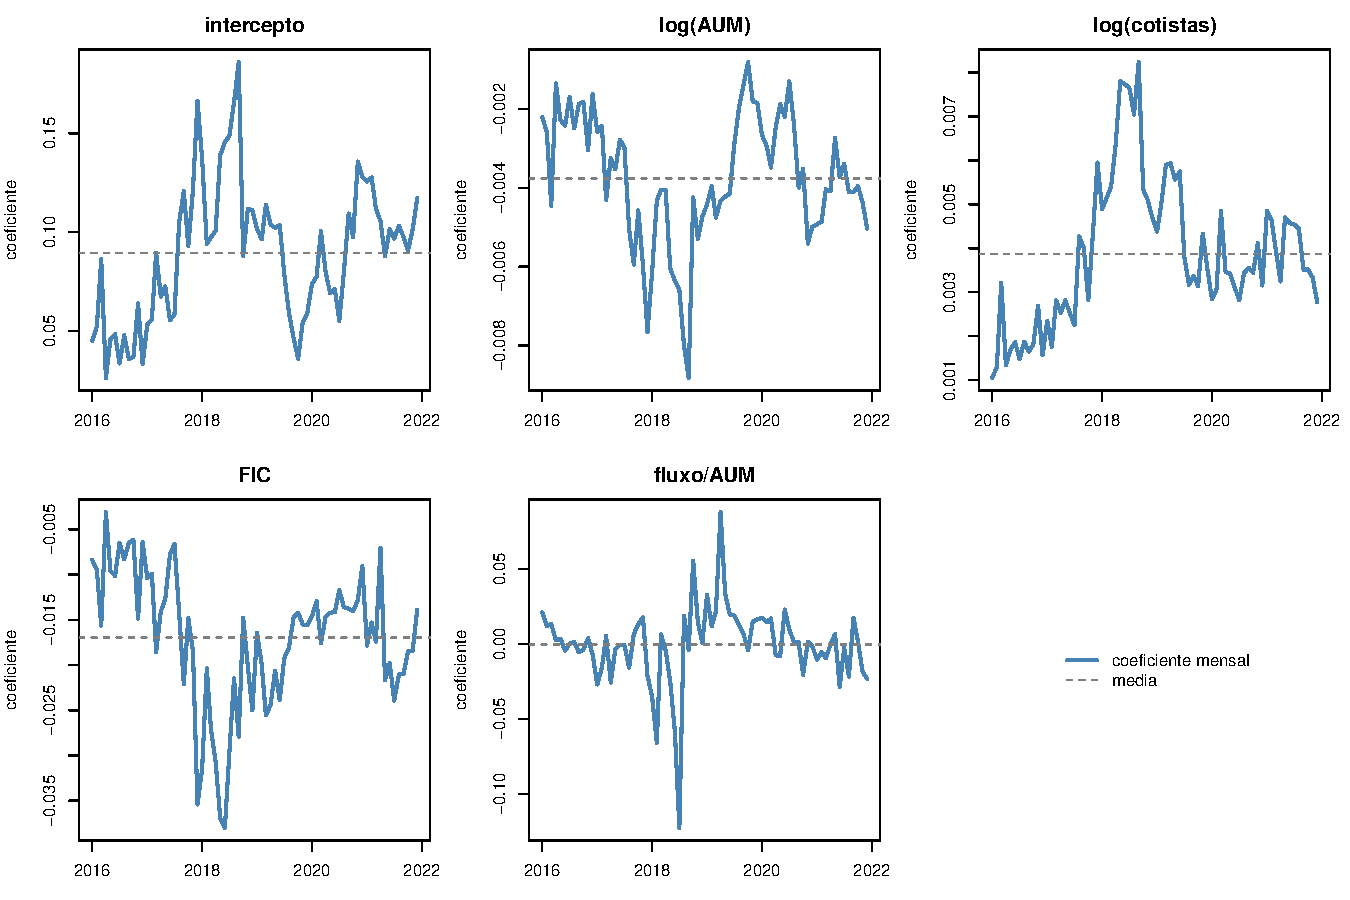
\includegraphics[width=\textwidth]{fig_theta.pdf}
\caption*{\footnotesize Séries dos coeficientes $\theta_t$ (2016--2021); linha
tracejada = média. Os fatores estruturais oscilam em torno de um nível estável
(reversão à média); o do fluxo é mais errático.}
\end{figure}

\section{Próximo passo}

Modelar a dinâmica via \textbf{estado-espaço / filtro de Kalman} com transição
AR(1) (ou nível local), que estima o caminho dos $\theta_t$ suavizando o ruído
amostral das estimativas mensais, liga o nível médio a preço e beta, e gera
previsão multi-horizonte do peso. Em seguida, a análise da matriz de erros.

\end{document}
